\section{Appendix}\label{sec:appendix}

This section acts as an appendix and explain an example Classifier program in Proximate space.  

\begin{figure}[h]
  \begin{center}
    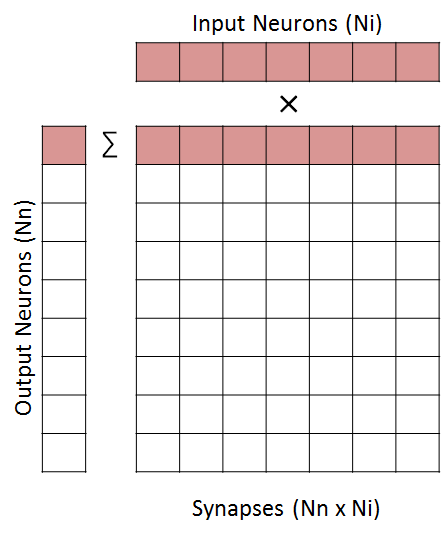
\includegraphics[width=0.3\linewidth]{cs758-figs/classifier-diagram.png}
  \end{center}
\vspace{-0.2in}
  \caption{Classifier workload diagram}
  \label{fig:classifier-diagram}
\vspace{-0.05in}
\end{figure}

Figure~\ref{fig:classifier-diagram} shows the classifier workload. 
Classifier requires multiplying the input neurons (a vector) by synapses 
(a matrix) and then doing the summation reduction.


\begin{figure}
  \begin{center}
    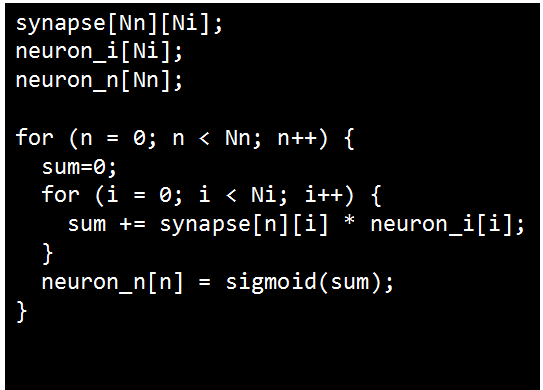
\includegraphics[width=0.5\linewidth]{cs758-figs/classifier-cpu.png}
  \end{center}
\vspace{-0.2in}
  \caption{Classifier implementation using sequential CPU}
  \label{fig:classifier-cpu}
\vspace{-0.05in}
\end{figure}

Figure~\ref{fig:classifier-cpu} shows the sequential implementation of 
classifier. Classifier can be done with a nested for loop to take the 
summation of the product between the input neurons and synapses.


\begin{figure}[h]
  \begin{center}
    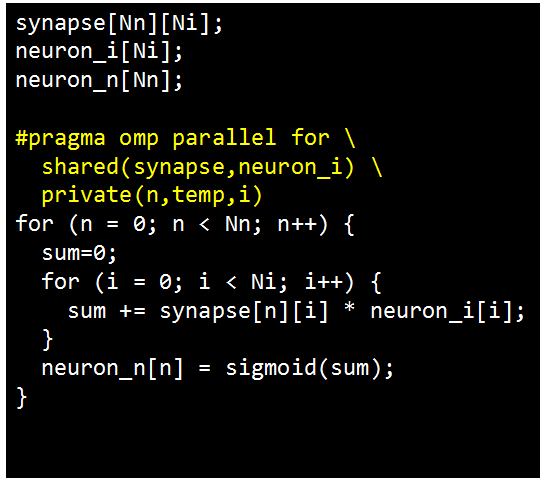
\includegraphics[width=0.5\linewidth]{cs758-figs/classifier-omp.png}
  \end{center}
\vspace{-0.2in}
  \caption{Classifier implementation using OpenMP}
  \label{fig:classifier-omp}
\vspace{-0.05in}
\end{figure}

Figure~\ref{fig:classifier-omp} shows the OpenMP implementation of 
classifier. The OpenMP implementation of classifier is using a 
\emph{\#pragma omp parallel} on the outer loop. 


\begin{figure}[h]
  \begin{center}
    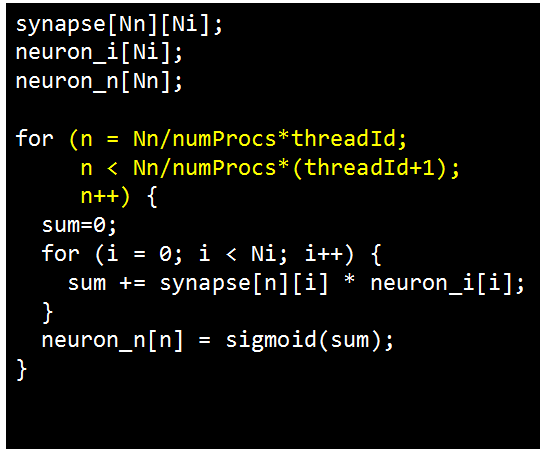
\includegraphics[width=0.5\linewidth]{cs758-figs/classifier-pthread.png}
  \end{center}
\vspace{-0.2in}
  \caption{Classifier implementation using pthreads}
  \label{fig:classifier-pthread}
\vspace{-0.05in}
\end{figure}

\paragraph{}

Figure~\ref{fig:classifier-pthread} shows the pthread implementation of 
classifier. The pthreads implementation of classifier shards the 
workload among pthreads. 


\begin{figure}
  \begin{center}
    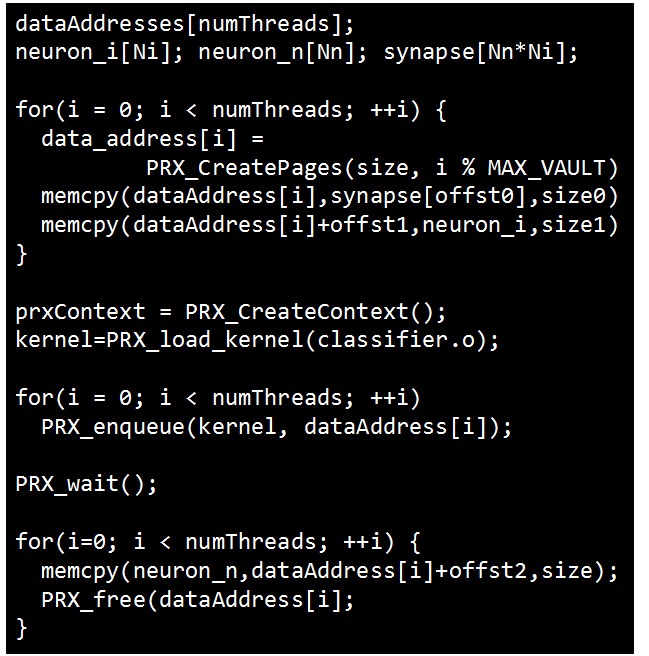
\includegraphics[width=0.5\linewidth]{cs758-figs/classifier-prx_inorder_q.png}
  \end{center}
\vspace{-0.2in}
  \caption{Classifier implementation using proximate with inorder cores and queuing model}
  \label{fig:classifier-prx_inorder_q}
\vspace{-0.05in}
\end{figure}

Figure~\ref{fig:classifier-prx_inorder_q} shows the proximate implementation 
with inorder cores and queuing model of classifier. The proximate queuing 
implementation of classifier shards the 
workload to different vaults. Calling create context 
will spawn threads to monitor work queues. Then, load the kernel so that each thread
know which kernel to execute upon receiving their thread arguments. 
Next, enqueue the workloads and wait for them to finish. 
Finally, gather the results back into a single array. 


\begin{figure}
  \begin{center}
    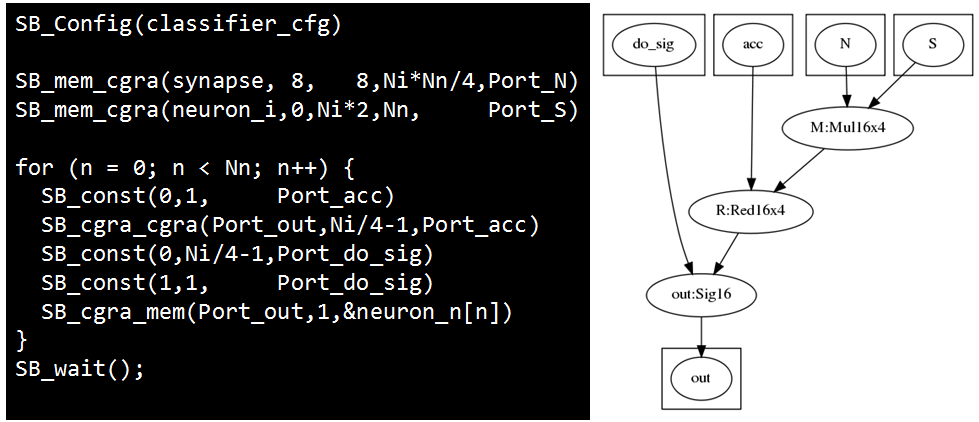
\includegraphics[width=\linewidth]{cs758-figs/classifier-prx_sb_only.png}
  \end{center}
\vspace{-0.2in}
  \caption{Classifier implementation using proximate with softbrain only}
  \label{fig:classifier-prx_sb_only}
\vspace{-0.05in}
\end{figure}

Figure~\ref{fig:classifier-prx_sb_only} shows the proximate implementation 
with softbrain only of classifier. The softbrain implementation first configures the
hardware to handle classifier. Then, pass inputs and synapses into softbrain. 
Loop through the softbrain fabric to do multiple iterations of the computation, one for each output.
Finally, wait for the softbrain computational fabric to finish. 
